\documentclass[12pt, a4paper]{article}
% There are different classes like:
% 1) article : for papers and reports
% 2) book : for books
% 3) letter: for letters
% 12pt (default 10pt) defines the fontsize for the whole article.
% letterpaper (default) defines the size of the paper, a4paper can also be used.

\usepackage{graphicx}
% latex package to import graphics for pictures

\usepackage{enumitem}

\usepackage{hyperref}
% For hyperlinks
\hypersetup{
    colorlinks=true,
    linkcolor=blue,
    filecolor=magenta,      
    urlcolor=cyan,
    pdftitle={Overleaf Example},
    pdfpagemode=FullScreen,
}

\usepackage{geometry}
% Page setup
\geometry{margin=1.2in}
\setlength{\parindent}{0pt}  % No paragraph indentation
\setlength{\parskip}{0em}  % Paragraph spacing


\usepackage{multicol}
% For multiple columns 

\usepackage[normalem]{ulem}
% For underline
\graphicspath{{Images/}}
% defining the path for images folder

\usepackage{tikz}
% For making curved arrows
\usepackage{float}

% Coding Template in Latex
\usepackage{listings}
\usepackage{color, soul}
\usepackage{xcolor}

\definecolor{dkgreen}{rgb}{0,0.6,0}
\definecolor{gray}{rgb}{0.5,0.5,0.5}
\definecolor{mauve}{rgb}{0.58,0,0.82}
\definecolor{grey}{rgb}{0.9,1,0.9}

\lstset{frame=tb,
  language=Verilog,
  aboveskip=3mm,
  belowskip=3mm,
  showstringspaces=false,
  columns=flexible,
  basicstyle={\small\ttfamily},
  numbers=left,
  numberstyle=\tiny\color{gray},
  keywordstyle=\color{blue},
  commentstyle=\color{dkgreen},
  stringstyle=\color{mauve},
  breaklines=true,
  breakatwhitespace=true,
  backgroundcolor=\color{white},
  tabsize=3
}
% Can change the language using \lstset{language=Java}
% Coding Template ends here

\title{Summer Training Report}
\author{\\[-5ex] Vedant Pahariya | Priyanshi Jain}
\date{}

\begin{document}
\maketitle
\tableofcontents
\newpage

% About the Title

\section{TinyML}
Reference: \href{https://www.datacamp.com/blog/what-is-tinyml-tiny-machine-learning}{What is TinyML?}  by datacamp

Many Machine learning applications require a lot of computational power and memory. Because of this demand, they are usually run on powerful servers or cloud computing platforms. 
\vspace{1em} \\
\fbox{
    \begin{minipage}{0.9\textwidth}
        In machine learning, the workflow consists of two main phases:
            \begin{itemize}[nosep]
                \item \textbf{Training} - When the model learns from data by adjusting its parameters
            \item \textbf{Inference} - When the trained model is used to make predictions on new data
        \end{itemize}
    \end{minipage}
} \\

In addition to these models being computationally expensive to train, running inference on them is often quite expensive too because of following reasons:

\begin{itemize}[nosep]
    \item They require a lot of memory to store the model parameters
    \item They require a lot of computational power to run the model and make predictions
    \item More energy than tiny devices can provide
\end{itemize}

\vspace{1em}
If machine learning is to expand its reach and penetrate additional domains, a solution that allows machine learning models to run inference on smaller, more resource-constrained devices is required. The pursuit of this solution is what has led to the subfield of machine learning called Tiny Machine Learning (TinyML). 

\vspace{1em}
TinyML is a type of machine learning that allows models to run on smaller, less powerful devices. It involves hardware, algorithms, and software that can analyze sensor data on these devices with very low power consumption, making it ideal for always-on use-cases and battery-operated devices.

\vspace{1em}
Benefits of TinyML:
\begin{itemize}[nosep]
    \begin{minipage}[t]{0.45\textwidth}
        \item Latency
        \item Energy savings
    \end{minipage}
    \hfill
    \begin{minipage}[t]{0.45\textwidth}
        \item Reduced bandwidth
        \item Data privacy
    \end{minipage}
\end{itemize}

\section{Neural Networks}
Neural networks are also called artificial neural networks (ANNs). Put simply, neural networks form the basis of architectures that mimic how biological neurons signal to one another. 


\subsection{Non-Linearity}
Non-linearity is crucial in neural networks because it allows them to learn complex patterns in the data. Without non-linear activation functions, a neural network would essentially behave like a linear regression model, regardless of the number of layers it has. This means it could only learn linear relationships, which are often insufficient for real-world tasks.

What is the use of the activation function in a neural network? Why we need Non-Linearity?\\
Reference: \href{https://youtu.be/gmjzbpSVY1A?si=zNG1e_BFRNVhcYxt&t=370}{Watch here}

\vspace{0.5em}

As shown in the video above, using linear functions, we can't construct a complex function like sinosoidal function. The output of a linear function is always a straight line, irrespective of the no. of layers in the network, the final equivalent function boils down to simple y= mx+ c, which means it can only represent linear relationships between inputs and outputs. 
Common non-linear activation functions include:
\begin{itemize}[nosep]
    \item Sigmoid
    \item Tanh
    \item ReLU (Rectified Linear Unit)
\end{itemize}

\begin{figure}[h]   % h stands for here, t for top, b for bottom, p for page
    \centering
    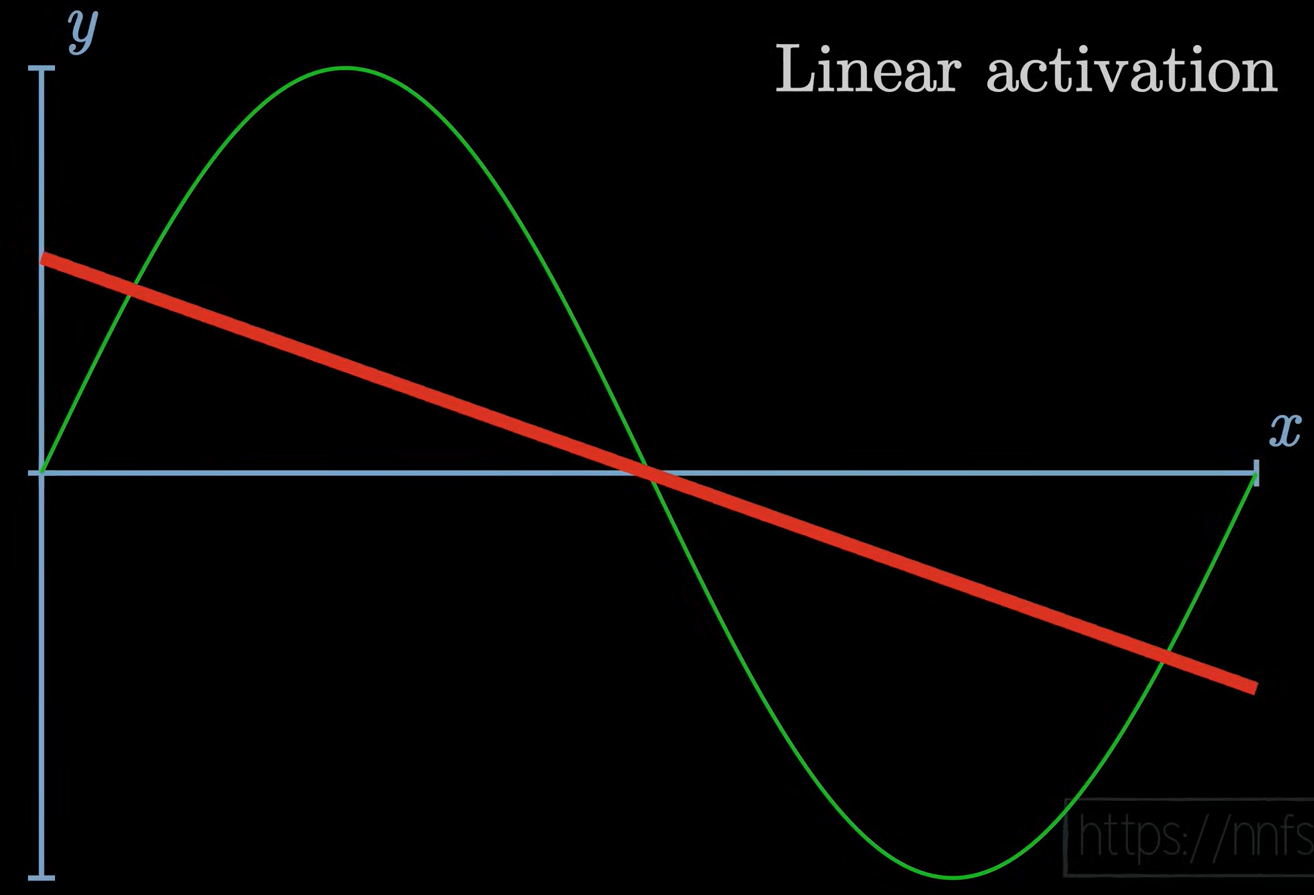
\includegraphics[width=0.5\textwidth]{Linear Activation.png} % width is in fraction of textwidth
    % \caption{Sample Image}% Caption of the image
    \label{fig:veri1}
\end{figure}

\subsection{Backpropagation}

Reference: \href{https://youtu.be/dB-u77Y5a6A?si=pFKasZnTR1_GaS5v}{Lecture by Justin Johnson}

\section{PyTorch}

Reference: \href{https://youtube.com/playlist?list=PLKnIA16_Rmvboy8bmDCjwNHgTaYH2puK7&si=q46c4wbwDzqZEilV}{Deep Learning using PyTorch - YouTube Playlist} 

\vspace{1em}

In 2002, Torch was a scientific computing framework with wide support for machine learning algorithms. 
But there were two problems in Torch: first, it is written in Lua, which is not widely used in the industry; second, it was using the static computational graph, which is not flexible and dynamic like PyTorch/ TensorFlow.

\vspace{0.5em}

These problems are fixed by PyTorch which is an open-source machine learning library developed by Facebook's AI Research lab. It is widely used for deep learning applications and provides a flexible and dynamic computational graph, making it easy to build and train neural networks.

\vspace{0.5em}

Core Features of PyTorch include:
\begin{itemize}[nosep]
    \item \textbf{Tensor Computations:} PyTorch provides a multi-dimensional array (tensor) library that is similar to NumPy but with GPU acceleration.
    \item \textbf{GPU Acceleration:} PyTorch can utilize GPUs for faster computation, making it suitable for deep learning tasks.
    \item \textbf{Dynamic Computation Graph:} PyTorch uses a dynamic computation graph, allowing for more flexibility in building and modifying neural networks.
    \item \textbf{Automatic Differentiation:} PyTorch uses a technique called automatic differentiation to compute gradients for high optimization tasks.
    \item \textbf{Distributed Training:} Training models on multiple GPUs or across multiple machines rather than a single GPU.
    \item \textbf{Interoperability with other libraries:} PyTorch can easily integrate with other popular libraries such as NumPy, SciPy, and Cython.
\end{itemize}

\subsection{What are Tensors?}

Tensors are a fundamental data structure in PyTorch, representing multi-dimensional arrays. They are similar to NumPy arrays but with additional capabilities for GPU acceleration and automatic differentiation. Tensors can be created from Python lists or NumPy arrays and can be manipulated using a variety of operations.

\vspace{0.5em}

\textbf{Examples:}
\begin{itemize}[itemsep=0.1em]
    \item \textbf{0D Tensor (Scalar):} A scalar tensor is a single value, which can be created from a Python number or a NumPy scalar. Output of Loss function is a scalar value.
    \item \textbf{1D Tensor:} A 1D tensor is an array or vector, which can be created from a Python list or NumPy array. The feauture vector of text is a 1D tensor, also known as embedding vector.
    \item \textbf{2D Tensor:} A 2D tensor is a matrix, which can be created from a list of lists or a 2D NumPy array. Gray Scale images are 2D tensors, where each pixel is represented by a single value like MNIST dataset.
    \item \textbf{3D Tensor:} A 3D tensor is a cube, which can be created from a list of 2D arrays or a 3D NumPy array. RGB images are 3D tensors, where each pixel is represented by three values (R, G, B).
    \item \textbf{4D Tensor:} A 4D tensor is a hypercube, which can be created from a list of 3D arrays or a 4D NumPy array. Video frames or Batch of RGB images are 4D tensors, where each frame is represented by a 3D tensor (RGB image).
    \item \textbf{5D Tensor:} Video data can be represented as a 5D tensor, where each frame is a 3D tensor (RGB image) and the batch size is the first dimension. For example, a batch of 10 video clips, each with 30 frames, can be represented as a 5D tensor with shape (10, 30, height, width, 3 RGB channels).
\end{itemize}

\subsection{Concept of seeding}

Seeding is a technique used to ensure that the random number generation in PyTorch is reproducible. By setting a seed value, we can ensure that the same random numbers are generated each time we run the code, which is useful for debugging and testing purposes.
A seed is a number that initializes the random number generator. If you use the same seed, you'll get the same sequence of random numbers.

\begin{center}
\begin{tabular}{|l|p{0.5\textwidth}|}
\hline
\textbf{Function} & \textbf{Purpose} \\
\hline
\texttt{torch.manual\_seed(seed)} & Sets the seed for \textbf{CPU} random number generation in PyTorch. \\
\hline
\texttt{torch.cuda.manual\_seed(seed)} & Sets the seed for \textbf{current GPU}. \\
\hline
\texttt{torch.cuda.manual\_seed\_all(seed)} & Sets the seed for \textbf{all GPUs}. \\
\hline
\texttt{torch.backends.cudnn.deterministic = True} & Forces cuDNN to use deterministic algorithms (slower, but reproducible). \\
\hline
\texttt{torch.backends.cudnn.benchmark = False} & Disables the auto-tuner that may introduce non-determinism. \\
\hline
\end{tabular}
\end{center}

\subsection{Autograd}

Autograd is PyTorch's automatic differentiation engine that powers neural network training. It allows us to compute gradients automatically, which is essential for optimizing model parameters during training.

Autograd keeps a record of data (tensors) and all executed operations in a directed acyclic graph (DAG) consisting of Function objects. \ul{For DAG, leaves are the input tensors, and roots are the output tensors}. By traversing this graph in reverse (backpropagation), we can compute gradients for all tensors involved in the computation.

\vspace{1em}

In a forward pass, autograd does two things simultaneously: \\
• run the requested operation to compute a resulting tensor\\
• maintain the operation's gradient function in the DAG.

\vspace{0.5em}

The backward pass kicks off when . backward() is called on the DAG root. autograd then:\\
• computes the gradients from each .grad\_fn ,\\
• accumulates them in the respective tensor's . grad attribute \\
• using the chain rule, propagates all the way to the leaf tensors.

\vspace{1em}

\textbf{Clearing Gradients}

After the backward pass, it's important to clear the gradients of the model parameters to prevent accumulation from previous iterations. This is typically done using the following command:

\begin{verbatim}
{Leaf(input)_Variable_Name}.grad.zero_()
\end{verbatim}

The Underscore after zero indicates that the operation is done in-place. 

There is other command \texttt{optimizer.zero\_grad()} which is used to clear the gradients of all model parameters in a single call. This is often used in training loops to reset gradients before the next forward and backward pass.
This function sets the gradients of all model parameters to zero, ensuring that the next forward and backward pass starts with a clean slate.

\textbf{Stopping the Backpropagation}

After the model is trained, we may want to stop the backpropagation for certain tensors/operations. This can be done in three ways:

\begin{itemize}[nosep]
    \item \texttt{detach()} - Returns a new tensor that shares the same data but does not require gradients. This is useful when we want to use a tensor in a computation without tracking its gradients.
    \item \texttt{with torch.no\_grad():} - A context manager that temporarily disables gradient tracking. This is useful for inference or evaluation, where we don't need to compute gradients.
    \item \texttt{requires\_grad=False} - Setting this attribute on a tensor prevents it from being included in the computation graph and stops gradient tracking for that tensor.
\end{itemize}

% example
\begin{lstlisting}[language=Python]
import torch
# Create a tensor with requires_grad=True
x = torch.tensor([1.0, 2.0, 3.0], requires_grad=True)
# Perform some operations
y = x * 2 + 1
# Compute gradients
y.backward(torch.tensor([1.0, 1.0, 1.0]))  # Backpropagate
print(x.grad)  # Print gradients
# Detach the tensor from the computation graph
x_detached = x.detach()  # Detach x from the graph
# Perform operations without tracking gradients
y_no_grad = x_detached * 2 + 1  # No gradients will be computed
# Use with torch.no_grad() context
with torch.no_grad():
    y_no_grad = x * 2 + 1  # No gradients will be computed
# Set requires_grad=False
x.requires_grad = False  # Stop tracking gradients for x
\end{lstlisting}

\subsection{Basics of OOPS in Python}

Reference: \href{https://www.youtube.com/watch?v=HQnoYzxOHMw}{Video-1} (Intro to OOPS) \href{https://youtu.be/a7baAGCBA9U?si=dic4GqzG0pJtPffX}{Video-2} (Classes \& Objects) \href{https://youtu.be/12HRkYld22c?si=2YsB6D_8Efi1Otr0}{Video-3} (Constructors)

\section{RISC-V}

RISC-V is an open standard instruction set architecture (ISA) based on established reduced instruction set computer (RISC) principles. The specification for this set of instructions is the 5th generation of RISC processors, which have been in development since the 1980s, thus we call it RISC-V. RISC-V ecosystem consists of following elements:
\begin{itemize}
    \item Physical hardware: Processors, development boards, System-on-Chips (SoCs), System-on-Modules (SoMs), and other physical systems.
    \item ``Soft'' IP processor cores that can be loaded into emulators, field-programmable gate arrays (FPGAs), or implemented in silicon.
    \item The entire software stack, from bootloaders and firmware, up to full operating systems and applications.
    \item Educational material including courseware, curricula, lesson plans, online courses like this one, tutorials, podcasts, lab assignments, and even books.
    \item Services including verification, custom board design, and many more.
\end{itemize} 

\subsection{RISC vs. CISC: Instruction Sets and Code Density}
RISC-V follows the RISC (Reduced Instruction Set Computer) philosophy, which contrasts with the CISC (Complex Instruction Set Computer) approach used in architectures like x86. A key distinction between these approaches involves two separate concepts that are often confused:

\begin{itemize}
    \item \textbf{Instruction Set Size}: The number of unique instruction types defined by the architecture
    \item \textbf{Instruction Count in Programs}: The number of instruction instances needed to implement a specific task
\end{itemize}

CISC architectures typically have \ul{\textit{larger} instruction sets (more unique instructions)} where \ul{most of which have access to memory} but require \ul{\textit{fewer} instructions to implement} a given program. For example, Intel's 80386 introduced in 1985 supported over 150 distinct instructions.

In contrast, RISC architectures like RISC-V have \ul{\textit{smaller} instruction sets (fewer unique instructions)} with \ul{memory access restricted to a few Load and Store instructions} but may require \ul{\textit{more} instructions to implement the same functionality}. The RISC-V base integer instruction set includes only 40 instructions.

\vspace{1em}
To illustrate this difference, consider a simple operation of adding a value from memory to a register:

\begin{center}
\begin{tabular}{|l|l|}
\hline
\textbf{CISC Approach} & \textbf{RISC Approach} \\
\hline
\texttt{ADD REG, [ADDR]} & \texttt{LOAD REG2, [ADDR]} \\
(One instruction) & \texttt{ADD REG1, REG1, REG2} \\
 & (Two instructions) \\
\hline
\end{tabular}
\end{center}

\vspace{1em}
This design choice in RISC architectures enables simpler hardware implementations, more efficient pipelining, and often better performance despite requiring more instructions to accomplish the same tasks. The tradeoff of using more, simpler instructions instead of fewer, complex instructions has proven beneficial for most modern processor designs.

Prof. Krste Asanović and graduate students Yunsup Lee and Andrew Waterman started the RISC-V instruction set in May 2010 as part of the Parallel Computing Laboratory (Par Lab) at UC Berkeley, of which Prof. David Patterson was Director. The Par Lab was a five-year project to advance parallel computing funded by Intel and Microsoft for \$10M over 5 years, from 2008 to 2013.

\subsection{RISC-V Name}
The name RISC-V was chosen to represent the fifth major RISC ISA design from UC Berkeley (RISC-I [15], RISC-II [8], SOAR [21], and SPUR [11] were the first four). We also pun on the use of the Roman numeral “V” to signify “variations” and “vectors”, as support for a range of architecture research, including various data-parallel accelerators, is an explicit goal of the ISA design.

\subsection{RISC-V Instruction Set Variants}
RISC-V is not just one instruction set, but a family of related ISAs. The core part of each ISA is called a base integer instruction set, and there are currently four main versions:

\begin{itemize}[nosep]
    \item \textbf{RV32I} – 32-bit registers and address space (XLEN = 32)
    \item \textbf{RV64I} – 64-bit registers and address space (XLEN = 64)
    \item \textbf{RV32E} – A smaller version of RV32I, with only 16 integer registers (instead of 32), made for small microcontrollers
    \item \textbf{RV128I} – A future version with 128-bit registers and address space (XLEN = 128)
\end{itemize}

All these versions use two's-complement to represent signed integers.
XLEN is the term used to refer to the register width (32, 64, or 128 bits).

\subsection{Shakti Processors}
Resources: \url{https://en.wikipedia.org/wiki/SHAKTI_(microprocessor)} \\
\url{https://github.com/platformio/platform-shakti} \\

Shakti is an Indian-developed, open-source RISC-V processor started as an academic initiative back in 2014 by the Reconfigurable Intelligent Systems Engineering (RISE) group at IIT-Madras. 

\subsubsection{Shakti Processor Variants}
The Shakti processor family includes several variants, each designed for different applications and performance levels. The variants are categorized into classes based on their intended use:
\begin{center}
\begin{tabular}{|l|p{0.7\textwidth}|}
\hline
\textbf{Variant} & \textbf{Description} \\
\hline
\textbf{E-class} & Embedded microcontroller class (RV32IMA), no MMU \\
\hline
\textbf{C-class} & Controller-class (with MMU), runs Linux \\
\hline
\textbf{I-class} & Industrial-class, superscalar \\
\hline
\textbf{M-class} & Multicore high-performance \\
\hline
\textbf{S-class} & Server-grade \\
\hline
\textbf{H-class} & High-performance, out-of-order execution \\
\hline
\end{tabular}
\end{center}

There are experimental variants as well, such as the Shakti H-class, which is a high-performance processor with out-of-order execution capabilities.


\subsection{Vega Processors}
Resources: \url{https://en.wikipedia.org/wiki/VEGA_Microprocessors} \\

Vega processors are developed by the Centre for Development of Advanced Computing (C-DAC) in India.
% Vega is India's first indigenous 64-bit Multi-core RISC-V based Superscalar Out-of-Order Processor

An out-of-order processor is a type of processor that executes instructions in a different order than they are written in the program, as long as it maintains the correct order of execution to ensure the program works correctly.
\subsubsection{Vega Processor Variants}
The Vega processor family includes several variants:

\begin{center}
\begin{tabular}{|l|p{0.7\textwidth}|}
\hline
\textbf{Variant} & \textbf{Description} \\
\hline
\textbf{Vega ET1031} & Embedded 32-bit processor with floating-point unit (FPU) support \\
\hline
\textbf{Vega ET1040} & Higher performance variant with memory management unit (MMU) \\
\hline
\textbf{Vega AS1061} & Security-focused variant with enhanced protection features \\
\hline
\end{tabular}
\end{center}

The Vega Series is entirely open-source and compatible with multiple toolchains, making it flexible for various development environments.

\section{SystemVerilog}

Refer: \href{https://youtube.com/playlist?list=PLqPfWwayuBvMwUjNHfyaX6CTK2KbeL2ga&si=NyddrPqUN_h-WrtD}{Youtube Playlist}\\
EDA Playground Link for Practicing : \url{https://edaplayground.com/x/t7M2}

Drawback of Verilog: Not able to extensively verify the design. Missing the Corner Cases

\subsection{About RTL}

Refer: \href{https://www.reddit.com/r/vlsi_enthusiast/comments/1ffoqd4/what_is_rtl_register_transfer_level_design_in_vlsi/}{Reddit Post}\\ 

RTL stands for Register Transfer Level, which is a design abstraction used in digital circuit design. The above Reddit post link gives the detailed RTL description, its uses and importance in VLSI design.

\subsection{Verilog Vs SystemVerilog}

Refer: \href{https://www.reddit.com/r/Verilog/comments/oqkcj5/difference_between_verilog_and_system_verilog/}{Reddit Post}\\ 

Verilog is subset of SystemVerilog. SystemVerilog is an extension of Verilog that includes additional features and capabilities, particularly for verification and design abstraction. Refer the above Reddit post for more details.\\

Think of SystemVerilog as C++ and Verilog as C. Everything you can write in C will work in C++, but C++ offers much more.\\

Vanilla Verilog is the pure, standard Verilog — without any SystemVerilog features. When someone says "vanilla Verilog", they usually mean "just Verilog, no SystemVerilog".


\subsection{Data Types}
Recalling for the data types in Verilog, we have reg, wire, integer, time, real etc. All these are 4-state data types, meaning they can take values 0, 1, X (unknown), and Z (high impedance).

In case of SystemVerilog, we have the following data types:

\begin{center}
\begin{tabular}{|l|l|p{0.5\textwidth}|}
\hline
\textbf{Data Type} & \textbf{States} & \textbf{Description} \\
\hline
\texttt{logic} & 4-state & Can be used in both procedural and continuous assignments (one at a time) \\
\hline
\texttt{bit} & 2-state & Can only take values 0 or 1, more efficient for synthesis \\
\hline
\texttt{enum} & Variable & Enumerated data type allowing named constant values \\
\hline
\texttt{struct} & Variable & Composite data type grouping related variables \\
\hline
\texttt{typedef} & N/A & User-defined type declarations for code reusability \\
\hline
\end{tabular}
\end{center}

Values of \texttt{reg} can only be assigned in procedural blocks like \texttt{always}  and \texttt{initial} blocks, while \texttt{wire} can only be assigned in continuous assignments using assign statements. Sometimes, we get confused between what to use (\texttt{wire} or \texttt{reg}) when and where. So to avoid this confusion, we can use  \texttt{logic} data type in SystemVerilog, which can be used in both procedural and continuous assignments (one at a time).

\vspace{1em}

Defining a variable as \texttt{logic} will let us use it in either procedural blocks (like \texttt{always} or \texttt{initial}) or continuous assignments (like \texttt{assign} statements).

\textbf{Example Usage:}
\begin{lstlisting}[language=Verilog]
// SystemVerilog logic data type
logic [7:0] data_bus;    // Can be used flexibly
logic       clock;       // Single bit logic

// Traditional Verilog approach
reg  [7:0] data_reg;     // Only in procedural blocks  
wire [7:0] data_wire;    // Only in continuous assignments
\end{lstlisting}

default value of both \texttt{reg} and \texttt{logic} is \texttt{X} (unknown) in simulation.

\subsubsection{2-State Data Types}
These data types can only take values 0 or 1, making them more efficient for synthesis and simulation. Following are the 2-state data types in SystemVerilog:

\begin{center}
\begin{tabular}{|l|p{0.7\textwidth}|}
\hline
\textbf{Data Type} & \textbf{Description} \\
\hline
\texttt{bit} & Unsigned single bit data type that can take values 0 or 1. \\
\hline
\texttt{byte} & An 8-bit signed data type that can take values from -128 to 127. It is a convenient way to represent small integers. \\
\hline
\texttt{shortint} & A 16-bit signed integer data type that can take values from -32768 to 32767. It is useful for representing small signed integers. \\
\hline
\texttt{int} & A 32-bit signed integer data type that can take values from -2147483648 to 2147483647. It is the default integer type in SystemVerilog. \\
\hline
\texttt{longint} & A 64-bit signed integer data type that can take values from -9223372036854775808 to 9223372036854775807. It is useful for representing large signed integers. \\
\hline
\end{tabular}
\end{center}

\textbf{Important Note:} What will happen if we assign x or z to these 2-state data types?

If x or z values are assigned to 2-state data types, then it will be automatically converted to 0.

\subsubsection{Struct Data Type}
The difference between \texttt{struct} and \texttt{array}
is that grouping of different data types in \texttt{struct} while \texttt{array} is grouping of same data types.

\vspace{1em}
Following is the syntax for defining a struct in SystemVerilog:

\begin{lstlisting}[
    language=Verilog,
    backgroundcolor={\color{gray!10}},
    firstnumber=1,
    % nolol=true
    ]
    // SystemVerilog struct data type
    struct packed {
        logic [7:0] data;  // 8-bit data field
        logic valid;       // Validity flag
    } my_struct;          // Instance of the struct

    // Accessing struct fields
    my_struct.data = 8'hFF;  // Assigning value to data field
    my_struct.valid = 1'b1;  // Assigning value to valid field
    // Using struct in a module
\end{lstlisting}

\textbf{Packed vs Unpacked Structs:}

Above code defines a \textit{packed} struct in SystemVerilog. 

Packed structs are stored in a contiguous block of memory, with no padding between fields. This makes them more efficient for hardware representation. Good for synthesizable code or bit-level operations.

\vspace{1em}

Unpacked structs, on the other hand, allow for padding and can have variable-sized fields. They are more flexible but less efficient for hardware representation. Each member may be separately stored.

\begin{lstlisting}[
    language=Verilog,
    backgroundcolor={\color{gray!10}},
    firstnumber=1,
    % nolol=true,
    title={Packed vs Unpacked Structs}
]
    typedef struct packed {           |     typedef struct {
      logic [3:0] a;                  |       logic [3:0] a;
      logic [3:0] b;                  |       logic [3:0] b;
    } my_struct_t;                    |     } my_struct_t;
    +----------+----------+
    | bits 7:4 | bits 3:0 |
    |    a      |    b      |
    +----------+----------+
\end{lstlisting}

\vspace{1em}

\textbf{Using Typedef}

Typedef allows us to create new data types based on existing ones. This can help improve code readability and maintainability by giving meaningful names to complex data types.


\begin{lstlisting}[
    language=Verilog,
    backgroundcolor={\color{gray!10}},
    firstnumber=1,
    % nolol=true,
    title={Verilog Code using Typedef}
    ]
    logic [7:0] byte_t;               |     typedef logic [7:0] byte_t;  
    // Here, byte_t is a variable     |     // Define a new type byte_t
    logic [7:0] data1;                |     byte_t data1;     
    logic [7:0] data1;                |     byte_t data2;   
                                      |     // variables of type byte_t
\end{lstlisting}


\textbf{Good Example}

\begin{lstlisting}[
    language=Verilog,
    backgroundcolor={\color{gray!10}},
    firstnumber=1,
    % nolol=true,
    title={Good Example of Packed Struct Usage with Typedef}
]
    typedef struct packed {
        logic [3:0] a;
        logic [3:0] b;
    } my_struct_t;

    my_struct_t s;
    initial begin
    s = 8'b10001100; // assign whole struct as 8-bit value
    end
\end{lstlisting}

In the above example, the packed struct \texttt{my\_struct\_t} is defined with two 4-bit fields \texttt{a} and \texttt{b}. The struct can be assigned a single 8-bit value where first four bits correspond to \texttt{a} and the last four bits correspond to \texttt{b}. So here, a= 1000 (8) and b=1100 (12).

\vspace{1em}

\subsubsection{Enumerated Data Types}

Enumerated data types allow us to define a set of named values, which can make our code more readable and maintainable. They are particularly useful for representing states or modes in our design.

\begin{lstlisting}[
    language=Verilog,
    backgroundcolor={\color{gray!10}},
    firstnumber=1,
    % nolol=true,
    title={Enumerated Data Type Example}
]
    typedef enum {IDLE, RUNNING, DONE} state_t; // Define an enumerated type
    state_t current_state; // Declare a variable of the enumerated type
    // current state is a variable of enum data type which can take values IDLE, RUNNING, or DONE
    initial begin
        current_state = IDLE; // Assign a named value to the variable
    end
\end{lstlisting}

\subsubsection{Fixed Arrays (Packed/Unpacked)}

Arrays in SystemVerilog can be one-dimensional or multi-dimensional, and they can be packed or unpacked. Packed arrays are stored in a contiguous block of memory, while unpacked arrays allow for variable-sized elements. 

Packed arrays are typically used when you need to manipulate the entire array as a single unit at bit level operations, particularly for tasks like bit slicing or packing/unpacking data.

\textbf{Note:} Packed arrays have restrictions on the data types they can use. We cannot use the 2-state data types like \texttt{int}, \texttt{byte}, \texttt{shortint}, or \texttt{longint} with packed arrays. \ul{Packed arrays can only be used with data types like \texttt{logic}, \texttt{bit}, and \texttt{enum}.}

\vspace{1em}

\textbf{Example of Packed Array:} 
Following is the syntax for one-dimensional two bit packed array:
\begin{lstlisting}[
    backgroundcolor={\color{grey}},
    frame= none,
    numbers=none,
    xleftmargin=.35\textwidth,
    xrightmargin=.3\textwidth, 
    ]
    bit [1:0] array;
\end{lstlisting}

\textbf{Note:} Here, we don't need to use the keyword \texttt{packed} explicitly like we did for structs.

\vspace{0.5em}
For multi-dimensional packed arrays, the data will be stored in contiguous memory locations only like in linear one dimensional fashion. The syntax for a two-dimensional packed array is as follows:

\begin{lstlisting}[
    backgroundcolor={\color{grey}},
    frame= none,
    numbers=none,
    xleftmargin=.35\textwidth,
    xrightmargin=.3\textwidth, 
    ]
    bit [1:0][2:0] array;
\end{lstlisting}

In unpacked arrays, the \ul{ array dimensions are mentioned after the variable name} and they \ul{can be of any data type} like \texttt{int}, \texttt{byte}, \texttt{shortint}, or \texttt{longint}.

\vspace{1em}

\textbf{Example of Unpacked Array:}
\begin{lstlisting}[
    backgroundcolor={\color{grey}},
    frame= none,
    numbers=none,
    xleftmargin=.35\textwidth,
    xrightmargin=.3\textwidth, 
    ]
    int array [1:0][2:0]; 
\end{lstlisting}

This defines a two-dimensional unpacked array where the first dimension has 2 elements and the second dimension has 3 elements. The data type of the elements is \texttt{int}.

\begin{lstlisting}[
    backgroundcolor={\color{grey}},
    frame= none,
    numbers=none,
    xleftmargin=.3\textwidth,
    xrightmargin=.25\textwidth, 
    ]
    bit [1:0] packed_array [3:0];
\end{lstlisting}

Here, we have defined a packed array named \texttt{packed\_array} with 4 elements, each of which is 2 bits wide. The elements can be accessed using indices like \texttt{packed\_array[0]}, \texttt{packed\_array[1]}, etc. It is packed along one dimension that is [1:0] is continuous memory locations but unpacked along the other dimension that is [3:0] is not continuous memory locations.

\textbf{Assigning Values to Arrays:}
\begin{lstlisting}[
    language=Verilog,
    backgroundcolor={\color{gray!10}},
    firstnumber=1,
    % nolol=true,
    title={Assigning Values to Array}
]
    int unpacked_array [3:0];           |    int unpacked_array [3:0];
    // 4 int elements                   |
    packed_array[0] = 2'b01;            |
    packed_array[1] = 2'b10;            |   unpacked_array = '{10,20,30,40};
    packed_array[2] = 2'b11;            |   // Use ' to assign values 
    packed_array[3] = 2'b00;            |   // directly to the entire array
\end{lstlisting}


In the above example, using apostrophe (') allows us to assign values directly to the entire array in one go. This is particularly useful for initializing arrays with known values. This will give unpacked\_array[0] = 40 unpacked\_array[1] = 30 and so on.

\vspace{1em}

\textbf{Accessing Array Elements:}

To access all elements of an array, we can use a \texttt{foreach} loop in SystemVerilog. This loop iterates over each element of the array, allowing us to perform operations on them. This is similar to the \texttt{for} loop in C/C++. We can also use \texttt{for} loop to access the elements of the array.
\begin{lstlisting}[
    language=Verilog,
    backgroundcolor={\color{gray!10}},
    firstnumber=1,
    % nolol=true,
    title={Accessing Array Elements using foreach}
]
    foreach (packed_array[i]) begin
        // Access each element of packed_array
        $display("Element %0d: %b", i, packed_array[i]);
    end

    // Using for loop to access elements
    for (int i = 0; i < $size(packed_array); i++) begin
        $display("Element %0d: %b", i, packed_array[i]);
    end
\end{lstlisting}

\textbf{Note:} The \texttt{foreach} loop is particularly useful for iterating over arrays with dynamic sizes, as it automatically adjusts to the size of the array.

\vspace{0.5em}

\textbf{Packed Array Example:}
\begin{lstlisting}[
    language=Verilog,
    backgroundcolor={\color{gray!10}},
    firstnumber=1,
    title={Packed Array Example}
]
module example;
    bit [2:0][3:0][7:0] data; 

    initial 
        begin
            data = 96'hffff_ffff_ffef_ffef_aaaa_aaaa_bbbb_bbbb;
            $display("the value of data is: %b", data);
            
            // Display array values
            foreach (data[i]) 
                begin
                    $display("data[%0d] = %b", i, data[i]);
                foreach (data[i][j]) 
                    begin
                        $display("data[%0d][%0d] = %b", i, j, data[i][j]);
                    end
                end
        end
endmodule
\end{lstlisting}

\textbf{Output:}
\vspace{-0.5em}
\begin{figure}[H]
    \centering
    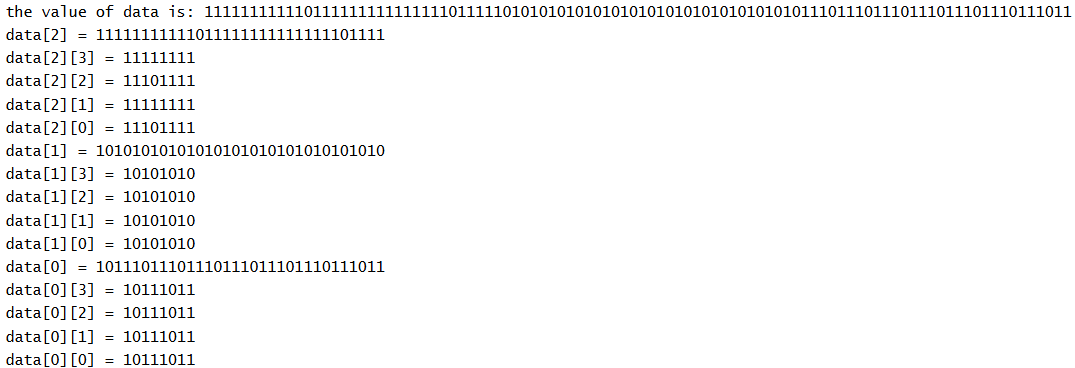
\includegraphics[width=1\textwidth]{Packed_Output.png}
\end{figure}

\subsubsection{Dynamic Arrays}

\textbf{Compile Time vs Runtime}

Compile-time refers to the phase in the development process when the source code is translated into machine code (or intermediate code) by a compiler. This phase happens before the program is run. The goal of compile-time activities is to check and transform the code so that it is ready for execution.

\vspace{0.5em}

In HDLs like SystemVerilog, compile-time refers to \ul{the time when the compiler checks for the syntax, and the HDL code is converted into a netlist} or hardware structure before execution of program.

\vspace{0.5em}

Runtime is the \ul{phase when the compiled code is executed on a computer or hardware}. During runtime, the program is running, and it can perform operations, access memory, produce output and interact with the user or other systems.

\vspace{1em}

Dynamic arrays are a type of array in SystemVerilog that can change size during simulation. They are particularly useful when the size of the array is not known at compile time and can be adjusted based on runtime conditions.

In case of Fixed Arrays, the size of the array is fixed at compile time, meaning it cannot be changed during runtime. Dynamic array do not have a fixed size at compile-time. The size is not known or set during compilation, and no memory is allocated for the array at this stage.

To declare a dynamic array, you use the following syntax:

\begin{lstlisting}[
    backgroundcolor={\color{grey}},
    frame= none,
    numbers=none,
    xleftmargin=.35\textwidth,
    xrightmargin=.3\textwidth, 
    ]
    int dynamic_array [];
\end{lstlisting}

In this example, we declare a dynamic array of integers. The size of the array can be set at runtime using the \texttt{new()} method:

\begin{lstlisting}[
    backgroundcolor={\color{grey}},
    frame= none,
    numbers=none,
    xleftmargin=.25\textwidth,
    xrightmargin=.2\textwidth, 
    ]
    dynamic_array = new[10]; // Create an array with 10 elements
\end{lstlisting}

Dynamic arrays can also be resized using the \texttt{resize()} method:

\begin{lstlisting}[
    backgroundcolor={\color{grey}},
    frame= none,
    numbers=none,
    xleftmargin=.25\textwidth,
    xrightmargin=.2\textwidth, 
    ]
    dynamic_array.resize(20); // Resize the array to 20 elements
\end{lstlisting}

\vspace{1em}
\textbf{Copying the elements of Dynamic Array:}

Without explicitly creating the memory for the second dynamic array, we can copy the elements of one dynamic array to another just by using the following syntax:
\begin{lstlisting}[
    backgroundcolor={\color{grey}},
    frame= none,
    numbers=none,
    xleftmargin=.22\textwidth,
    xrightmargin=.17\textwidth, 
    ]
    int dynamic_array2[] = dynamic_array; 
    // Copy elements to another dynamic array
\end{lstlisting}

If we make any changes to \texttt{dynamic\_array}, it will also affect \texttt{dynamic\_array2} because both arrays are pointing to the same memory location. If we want to create a separate copy of the array, we can use the \texttt{new()} method to create a new dynamic array and then copy the elements.
\vspace{1em}

\textbf{Increasing the size of Dynamic Array:}

There are two methods to increase the size of a dynamic array in SystemVerilog:
\begin{itemize}
    \item The existing elements will be deleted and size will be increased.
    \item The existing elements will remain as it is and size will be increased.
\end{itemize}

\begin{lstlisting}[
    language=Verilog,
    backgroundcolor={\color{gray!10}},
    firstnumber=1,
    % nolol=true,
    title={Resizing Dynamic Array}
    ]
    dyn1 = new[20];                         | dyn1 = new[20](dyn1);
  // Existing elements will be deleted      | // Existing elements will remain
                                            | // Size of dyn1 will be increased to 20
\end{lstlisting}

Lets say the initial size of dyn1 is 10, then after resizing it to 20, the first method will delete the existing 10 elements and create a new array of size 20. The second method will keep the existing 10 elements and increase the size to 20, leaving the last 10 elements uninitialized (default value is \texttt{0}).
\vspace{1em}

\textbf{Builtin  Functions for Dynamic Arrays:}
\begin{itemize}[nosep]
    \item \texttt{size()} - Returns the number of elements in the dynamic array.
    \item \texttt{delete()} - Deletes the dynamic array and frees up memory.
    \item \texttt{push\_back()} - Adds an element to the end of the dynamic array.
    \item \texttt{pop\_back()} - Removes the last element from the dynamic array.
\end{itemize}

\vspace{0.5em}

\href{https://vlsiverify.com/system-verilog/dynamic-array-in-sv/}{Here}
 is the link of good Dynamic Array example code.

\textbf{Dynamic Array Example:}



\subsubsection{Queue}
In SystemVerilog, a queue is a variable-size, ordered collection of homogeneous elements (all elements are of the same type). Unlike static arrays and dynamic arrays, the size of a queue can change dynamically during runtime as elements are added or removed. Queues provide a powerful, flexible data structure that operates like a FIFO (First In, First Out) or LIFO (Last In, First Out) mechanism depending on how you manipulate the elements.

\vspace{0.5em}

In dynamic arrays, we have to explicitly create the memory for the array using the \texttt{new()} method before inserting the elements, but in queues, we don't have to do that. Memory is allocated in the queue automatically when we add elements to them.

\textbf{Key Characteristics:}

\begin{itemize}[nosep]
    \item \textbf{Dynamic Size:} Queues can grow or shrink as needed as elements are deleted or inserted, allowing for flexible memory usage.

    \item \textbf{Operations:} Queues support various operations such as inserting, deleting elements to the front or back, and  querying the queue size.

    \item \textbf{Homogeneous Elements:} All elements in a queue must be of the same data type.
    \item \textbf{FIFO Behavior:} Elements are typically added to the end and removed from the front, following a first-in-first-out order.
\end{itemize}

Here is the general syntax for declaring a queue in SystemVerilog:
\begin{lstlisting}[
    backgroundcolor={\color{grey}},
    frame= none,
    numbers=none,
    xleftmargin=.3\textwidth,
    xrightmargin=.25\textwidth, 
    ]
    data_type queue_name [$];
\end{lstlisting}

For example, to declare a queue of integers, you would use:
\begin{lstlisting}[
    backgroundcolor={\color{grey}},
    frame= none,
    numbers=none,
    xleftmargin=.35\textwidth,
    xrightmargin=.3\textwidth, 
    ]
    int my_queue [$];
\end{lstlisting}
This creates a queue named \texttt{my\_queue} that can hold integers.

\textbf{Builtin Functions}

\vspace{0.2em}

\begin{itemize}[nosep]
    \item \texttt{size()} - Returns the number of elements in the queue.
    \item \texttt{insert(index, value)} - Inserts a value at the specified index in the queue.
    \item \texttt{delete(index)} - Deletes the value at specified index. In case if index is not mentioned, it deletes all elements in the queue and frees up memory.
    \item \texttt{push\_back(value)} - Adds an element to the end of the queue.
    \item \texttt{push\_front(value)} - Adds an element to the front of the queue.
    \item \texttt{pop\_front()} - Removes and returns the first element from the queue.
    \item \texttt{pop\_back()} - Removes and returns the last element from the queue.
\end{itemize}

\subsubsection{Associative Arrays}
As we have discussed earlier about dynamic arrays and fixed arrays, there we have allocate the fixed memory space either in the compile time or at the runtime irespective of the fact that we are using that memory or not. For example, if we declare a dynamic array of size 100, then 100 memory locations will be allocated for that array even if we are using only 10 elements in that array, remaining 90 elements are just waste of memory. 

\vspace{1em}

Associative arrays provide a way to store data where the index or key doesn't need to be an integer (can also be a string) and doesn't need to be consecutive, unlike dynamic arrays or fixed-size arrays. This makes them similar to dictionaries or maps in other programming languages. They are very useful when the index values are sparse or irregular, allowing flexible and dynamic data storage.

Following is the syntax for declaring an associative array in SystemVerilog:
\begin{lstlisting}[
    backgroundcolor={\color{grey}},
    frame= none,
    numbers=none,
    xleftmargin=.2\textwidth,
    xrightmargin=.15\textwidth, 
    ]
    data_type associative_array_name [key_type];
\end{lstlisting}

key\_type can be of any data type, including integers, strings, or enumerated types. \ul{* (Wildcard type) index type inferred at first use}.
data\_type is the data type of the elements stored in the associative array.

\vspace{0.5em}

For example, to declare an associative array of integers with string keys, you would use:
\begin{lstlisting}[
    backgroundcolor={\color{grey}},
    frame= none,
    numbers=none,
    xleftmargin=.13\textwidth,
    xrightmargin=.08\textwidth, 
    ]
module example;
    int marks[string];
    initial begin
        marks["Alice"] = 85;
        marks["Bob"] = 90;
        marks["Charlie"] = 78;
        
        $display("Alice's marks: %Od", marks["Alice"]);
        $display("Bob's marks: %Od", marks["Bob"]);
        $display("Charlie's marks: %Od", marks["Charlie"]);
    end
endmodule
\end{lstlisting}

\textbf{Builtin Functions}
\vspace{0.2em}
\begin{itemize}[nosep]
    \item \texttt{num()} - Returns the number of elements currently stored in the associative array.
    \item \texttt{first(var)} - Returns the first key in the associative array and stores it in the variable \texttt{var}.
    \item \texttt{last(var)} - Returns the last key in the associative array and stores it in the variable \texttt{var}.
    \item \texttt{next(key)} - Returns the next key after the specified key in the associative array.
    \item \texttt{prev(key)} - Returns the previous key before the specified key in the associative array.
    \item \texttt{delete(key)} - Deletes the element associated with the specified key.
    \item \texttt{exists(key)} - Checks if the specified key exists in the associative array.
\end{itemize}

\textbf{Example using next()}

\begin{lstlisting}[
    language=Verilog,
    backgroundcolor={\color{gray!10}},
    firstnumber=1,
    % nolol=true,
    title={Example using next()}
]
module associative_array();

  int fruits[string];  
  initial begin
    
    fruits= '{"apple":6,"orange":2, "guava":3, "watermelon": 9,"grape":1};
    begin
      string  f; // Default value of f would be lowest index i.e. "apple"
      while(fruits.next(f))
        $display(" Next fruit of is [%s] = %0d",f,fruits[f]);
        //It'll stop as it's not cyclic in nature unlike enum
    end
  end
endmodule
\end{lstlisting}

Output:\\
``` \\
  Next fruit of is [apple] = 6 \\
  Next fruit of is [grape] = 1 \\
  Next fruit of is [guava] = 3 \\
  Next fruit of is [orange] = 2 \\
  Next fruit of is [watermelon] = 9 \\
```

\subsubsection{Summary}

\begin{figure}[H]
    \centering
    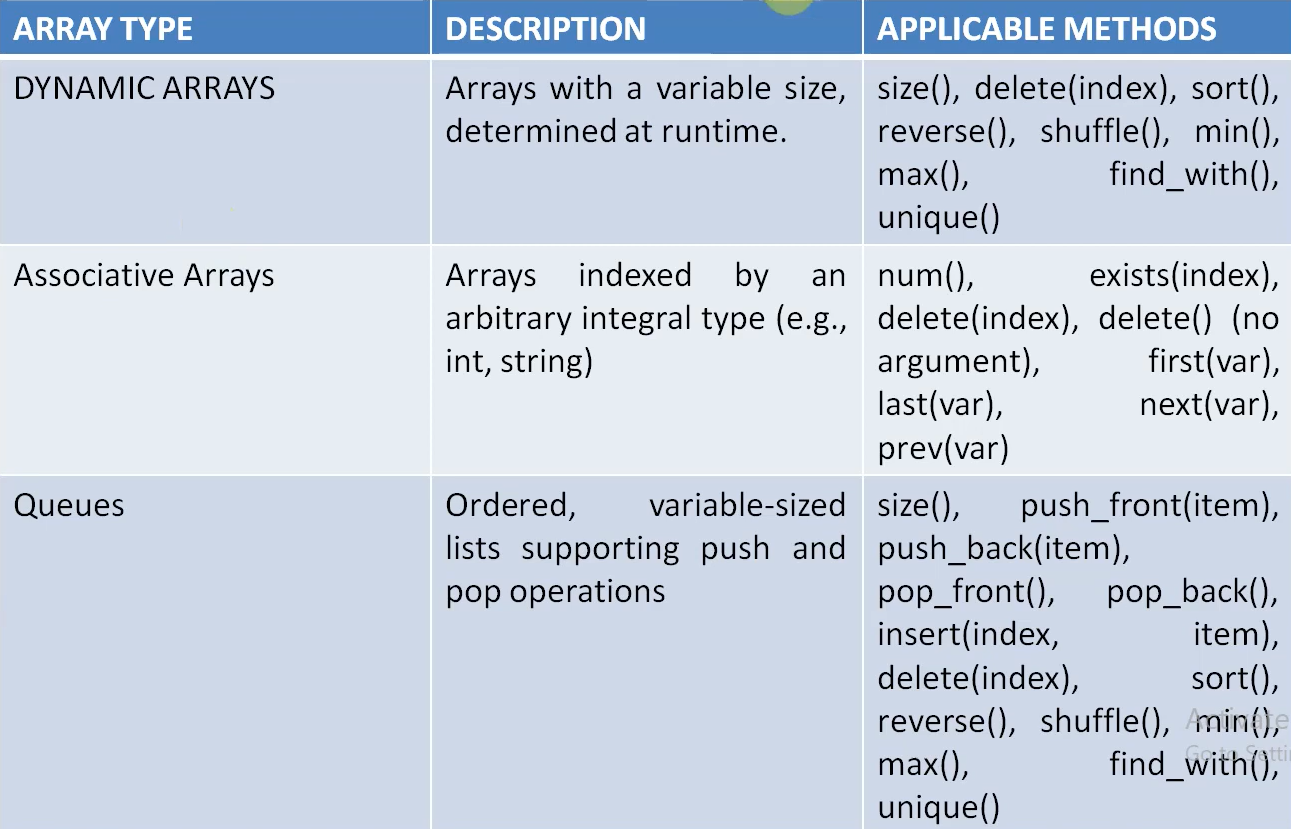
\includegraphics[width=0.8\textwidth]{DataTypes_sum1.png}
    % \caption{Summary of SystemVerilog Data Types}
    % \label{fig:data_types_summary}
\end{figure}
\vspace{-2em}
\begin{figure}[H]
    \centering
    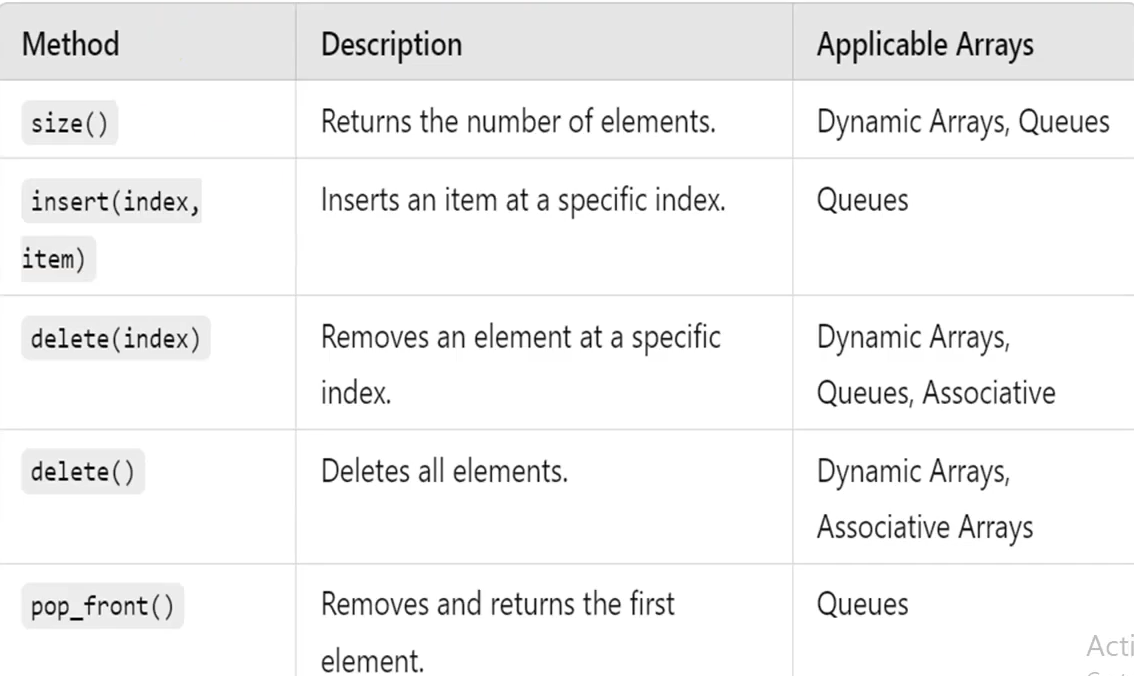
\includegraphics[width=0.8\textwidth]{DataTypes_sum2.png}
    % \caption{Summary of SystemVerilog Data Types (contd.)}
    % \label{fig:data_types_summary2}
\end{figure}
\vspace{-2em}
\begin{figure}[H]
    \centering
    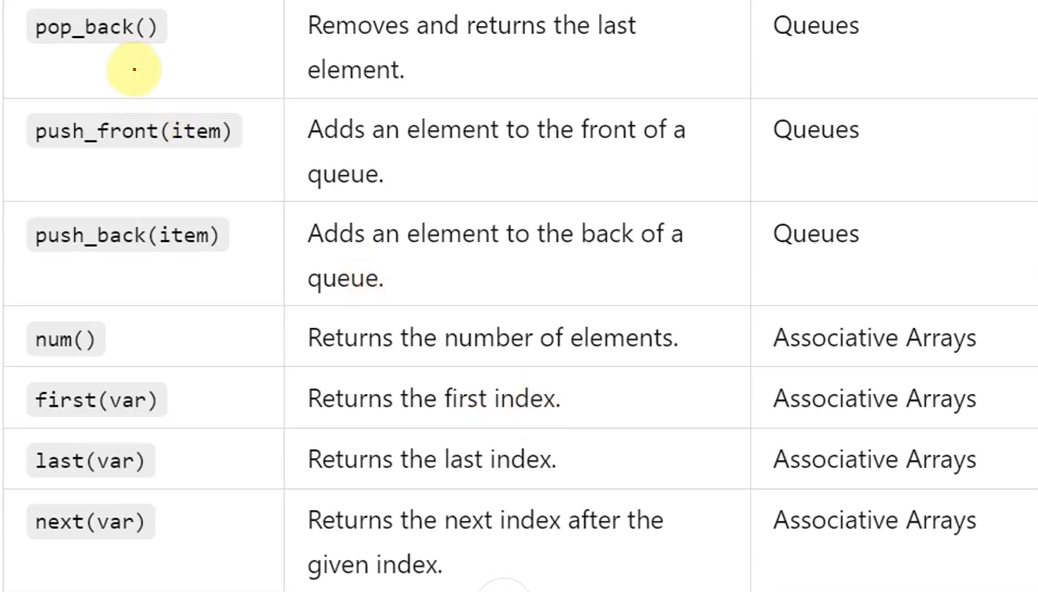
\includegraphics[width=0.8\textwidth]{DataTypes_sum3.png}
    % \caption{Summary of SystemVerilog Data Types (contd.)}
    % \label{fig:data_types_summary3}
\end{figure}
\vspace{-2em}
\begin{figure}[H]
    \centering
    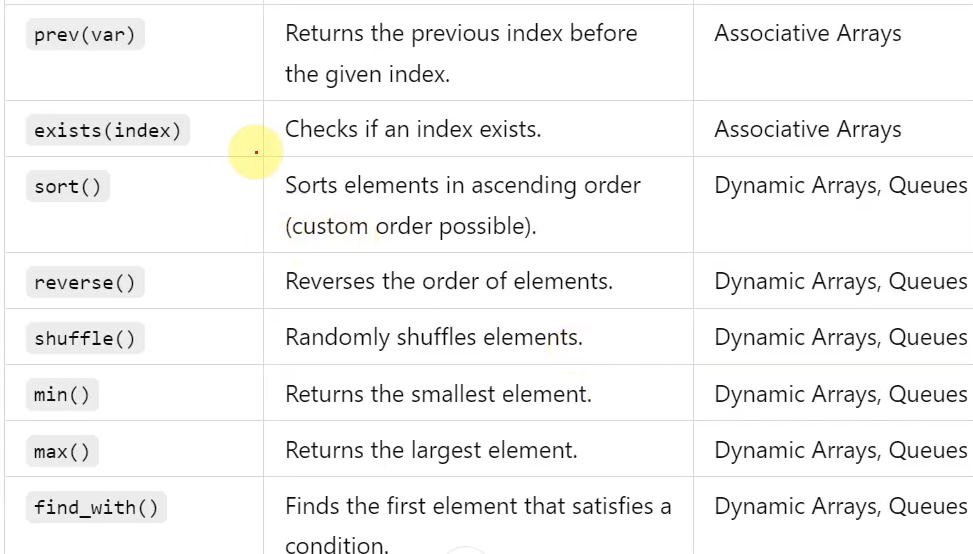
\includegraphics[width=0.8\textwidth]{DataTypes_sum4.png}
    % \caption{Summary of SystemVerilog Data Types (contd.)}
    % \label{fig:data_types_summary4}
\end{figure}

\subsection{Display Output}

In SystemVerilog, we can use the \texttt{\$display} function to print output to the console/Terminal. The \texttt{\$display} function is similar to the \texttt{printf} function in C/C++. It allows us to format the output and display variables, strings, and other data types.

\subsubsection{Format Specifiers}

The following table shows the format specifiers used with \texttt{\$display/\$write/\$monitor}  \texttt{/\$fwrite} in SystemVerilog:

\vspace{-1em}

\begin{center}
\begin{tabular}{|l|p{0.5\textwidth}|p{0.3\textwidth}|}
\hline
\textbf{Specifier} & \textbf{Meaning} & \textbf{Example Output} \\
\hline
\texttt{\%d} & Decimal (signed integer) & \texttt{42} \\
\hline
\texttt{\%0d} & Decimal with zero-padding (optional field width) & \texttt{00042} (if width is given) \\
\hline
\texttt{\%b} & Binary & \texttt{1010} \\
\hline
\texttt{\%h} & Hexadecimal & \texttt{A} \\
\hline
\texttt{\%o} & Octal & \texttt{12} \\
\hline
\texttt{\%c} & Character & \texttt{A} \\
\hline
\texttt{\%s} & String & \texttt{hello} \\
\hline
\texttt{\%t} & Time (used in simulations) & \texttt{\#100} \\
\hline
\texttt{\%\%} & Prints a literal \texttt{\%} & \texttt{\%} \\
\hline
\end{tabular}
\end{center}

\subsubsection{Zero-Padding/Space-Padding}

In SystemVerilog, we can also specify the width of the output and whether to use zero-padding or space-padding. The following table summarizes the different formats:

\vspace{-0.8em}

\begin{center}
\begin{tabular}{|l|l|p{0.4\textwidth}|}
\hline
\textbf{Format} & \textbf{Name} & \textbf{Example Output (for x = 7)} \\
\hline
\texttt{\%0d} & Zero-padding (no width → acts like \texttt{\%d}) & \texttt{7} \textit{(no padding seen)} \\
\hline
\texttt{\%04d} & Zero-padding with width & \texttt{0007} \\
\hline
\texttt{\%4d} & Space-padding (right-aligned) & \texttt{   7} \textit{(3 spaces before 7)} \\
\hline
\texttt{\%-4d} & Left-aligned space-padding & \texttt{7   } \textit{(3 spaces after 7)} \\
\hline
\end{tabular}
\end{center}


\section{CVA6}

References: \href{https://github.com/openhwgroup/cva6}{GitHub Repository}

\section{PULP-TrainLib}

\section{UVM}
Reference: \href{https://youtube.com/playlist?list=PLuYB6t6povcLgoHWLJgk-VeMQ0Rscjw03&si=l-rjyvLkuttomYeC}{Playlist1}
\href{https://youtube.com/playlist?list=PLqPfWwayuBvNrr09dCweog1htCBLUbN4W&si=4vI1Fs_sgz-A0wXdC}{Playlist2} are the links to the UVM playlists.

\section{On-Device Training}

% Basic Latex Template
\subsubsection{Subsection}

Introduce about the \underline{Title} here. \\

% Here is the way to attach the links in the document
Reference: \url{https://www.youtube.com/watch?v=ic1UMeuCBA8} \\
\href{https://www.geeksforgeeks.org/difference-between-gate-level-and-structural-verilog-hdl/}{GeeksforGeeks}

\begin{itemize}
    \item \textbf{1}: 
    \item \textbf{2}:
\end{itemize}

\begin{figure}[h]   % h stands for here, t for top, b for bottom, p for page
    \centering
    \includegraphics[width=0.65\textwidth]{example-image-a} % width is in fraction of textwidth
    \caption{Sample Image}% Caption of the image
    \label{fig:veri1}
\end{figure}

Verilog is a \underline{Case Sensitive} language. \\
The term ``module'' refers to the text enclosed by the keyword pair \textbf{module} \ldots \textbf{endmodule}. Module is the fundamental descriptive unit in Verilog language. \\
Keyword ``module'' is followed by the \underline{name of the design} (ABC here) and \uline{parenthesis - enclosed list of ports}.\\
% uline works better than underline when the text is being wrapped and going in the next line. 

\end{document}